\documentclass{beamer}
\usepackage[english, russian]{babel}
\usepackage[T2A]{fontenc}
\usepackage[utf8]{inputenc}
\usepackage{indentfirst}
\usepackage{amsmath, amsfonts, amssymb, amsthm, mathtools}
\usepackage[export]{adjustbox}
\usepackage{graphicx} 
\graphicspath{ {./images/} }

\usepackage{subcaption}
\usepackage{verbatim}

\usepackage{minted}{\setlength{\parskip}{0pt}}

\usepackage{hyperref}

\hypersetup{
    colorlinks=true,
    linkcolor=blue,
    filecolor=magenta,      
    urlcolor=black,
    pdftitle={Overleaf Example},
    pdfpagemode=FullScreen,
    }


\title{Лабораторная работа № 6. \\Установка и настройка системы управления базами данных MariaDB}
\author{Данила Стариков \\ НПИбд-02-22}
\institute{Российский университет дружбы народов имени Патриса Лумумбы}
\date{2024}

\begin{document}

\frame{\titlepage}

\begin{frame}
\frametitle{Цель работы}
\begin{itemize}
    \item Приобретение практических навыков по установке и конфигурированию системы управления базами данных на примере программного обеспечения MariaDB.
\end{itemize}
\end{frame}

\begin{frame}
\frametitle{Установка MariaDB}
    \centering
    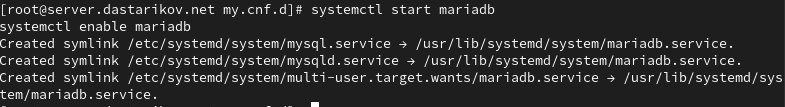
\includegraphics[width=\textwidth]{../images/image01.png}
    \captionof{figure}{Запуск ПО \texttt{mariadb}.}
\end{frame}

\begin{frame}
\frametitle{Установка MariaDB}
    \centering
    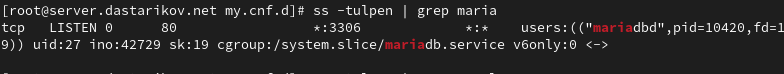
\includegraphics[width=\textwidth]{../images/image02.png}
    \captionof{figure}{Проверка прослушивания порта.}
\end{frame}

\begin{frame}
\frametitle{Установка MariaDB}
    \centering
    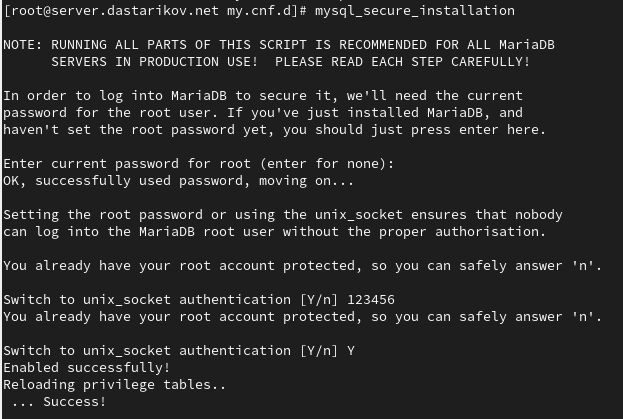
\includegraphics[width=\textwidth]{../images/image03.png}
    \captionof{figure}{Настройка конфигурации безопасности \texttt{mariadb}.}
\end{frame}

\begin{frame}
\frametitle{Установка MariaDB}
    \centering
    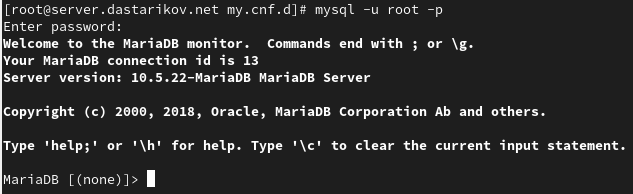
\includegraphics[width=\textwidth]{../images/image04.png}
    \captionof{figure}{Вход в базу данных с правами администратора.}
\end{frame}

\begin{frame}
\frametitle{Установка MariaDB}
    \centering
    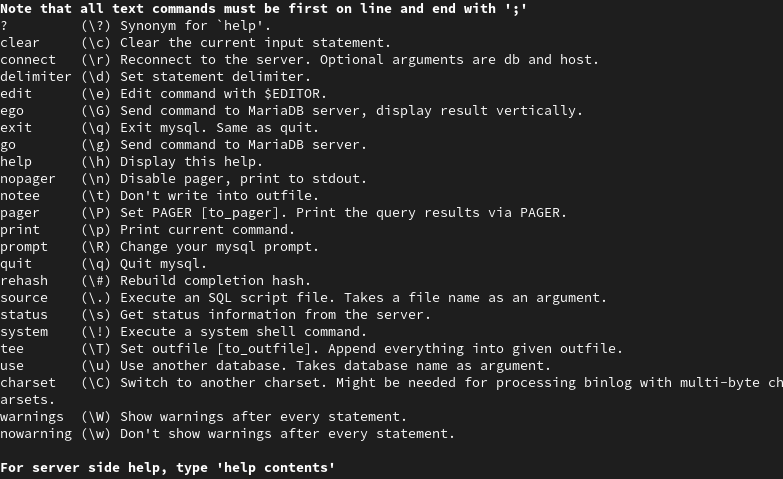
\includegraphics[width=\textwidth]{../images/image05.png}
    \captionof{figure}{Просмотр списка команд MySQL.}
\end{frame}

\begin{frame}
\frametitle{Установка MariaDB}
    \centering
    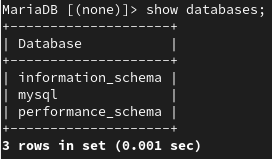
\includegraphics[width=\textwidth]{../images/image06.png}
    \captionof{figure}{Просмотр доступных баз данных.}
\end{frame}

\begin{frame}
\frametitle{Установка MariaDB}
    \centering
    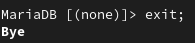
\includegraphics[width=\textwidth]{../images/image07.png}
    \captionof{figure}{Выход из интерактивной оболочки MariaDB.}
\end{frame}

\begin{frame}
\frametitle{Конфигурация кодировки символов}
    \centering
    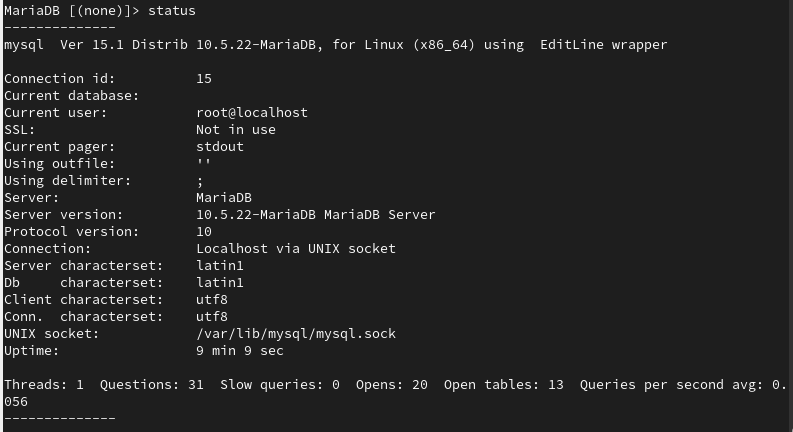
\includegraphics[width=\textwidth]{../images/image08.png}
    \captionof{figure}{Просмотр статуса MariaDB.}
\end{frame}

\begin{frame}[containsverbatim]
\frametitle{Конфигурация кодировки символов}
\begin{itemize}
\item В каталоге \texttt{/etc/my.cnf.d} создали файл \texttt{utf8.cnf}:
  \begin{minted}{bash}
    cd /etc/my.cnf.d
    touch utf8.cnf
  \end{minted}
  Открыли его на редактирование и указали в нём следующую конфигурацию:
  \begin{minted}{bash}
    [client]
    default-character-set = utf8
    [mysqld]
    character-set-server = utf8
  \end{minted}
\item Перезапустили MariaDB:
  \begin{minted}{bash}
    systemctl restart mariadb
  \end{minted}
\end{itemize}
\end{frame}

\begin{frame}
\frametitle{Конфигурация кодировки символов}
    \centering
    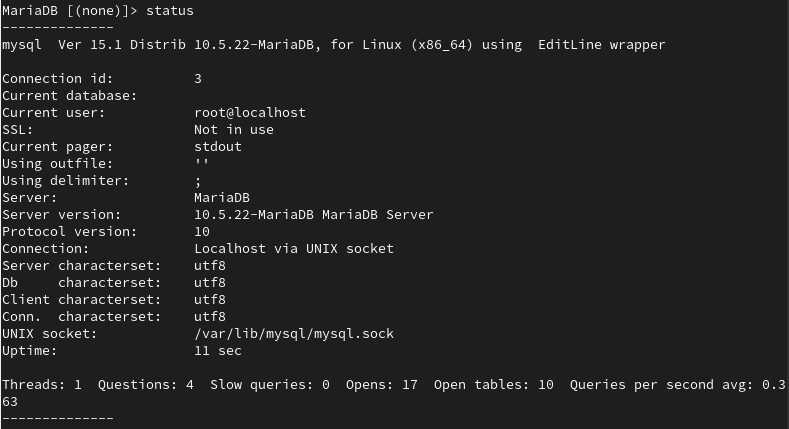
\includegraphics[width=\textwidth]{../images/image10.png}
    \captionof{figure}{Просмотр статуса MariaDB после изменения конфигурации.}
\end{frame}

\begin{frame}
\frametitle{Создание базы данных}
    \centering
    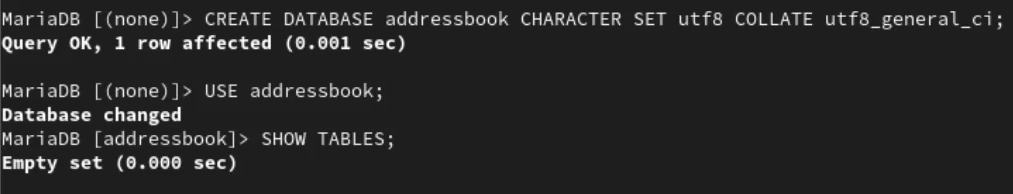
\includegraphics[width=\textwidth]{../images/image21.png}
    \captionof{figure}{Создание базы данных \texttt{addressbook}.}
\end{frame}

\begin{frame}
\frametitle{Создание базы данных}
    \centering
    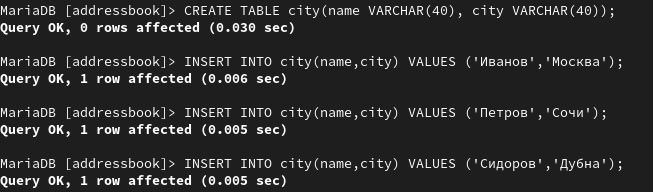
\includegraphics[width=\textwidth]{../images/image11.png}
    \captionof{figure}{Создание и заполнение таблицы.}
\end{frame}

\begin{frame}
\frametitle{Создание базы данных}
    \centering
    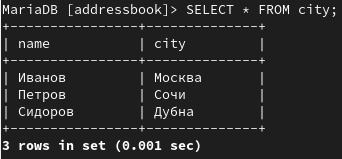
\includegraphics[width=\textwidth]{../images/image12.png}
    \captionof{figure}{Просмотр вхождений таблицы.}
\end{frame}

\begin{frame}
\frametitle{Создание базы данных}
    \centering
    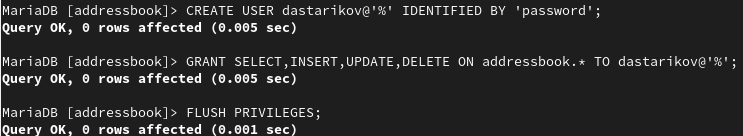
\includegraphics[width=\textwidth]{../images/image13.png}
    \captionof{figure}{Создание нового пользователя для работы с таблицей.}
\end{frame}

\begin{frame}
\frametitle{Создание базы данных}
    \centering
    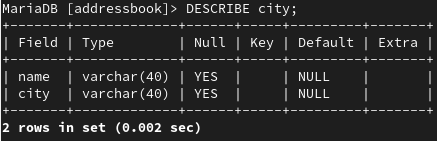
\includegraphics[width=\textwidth]{../images/image14.png}
    \captionof{figure}{Общая информация о таблице.}
\end{frame}

\begin{frame}
\frametitle{Создание базы данных}
    \centering
    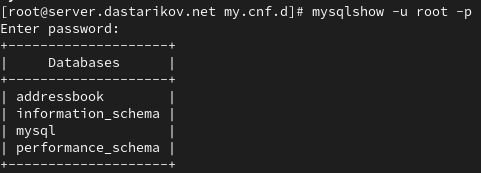
\includegraphics[width=\textwidth]{../images/image15.png}
    \captionof{figure}{Просмотр списка баз данных.}
\end{frame}

\begin{frame}
\frametitle{Создание базы данных}
    \centering
    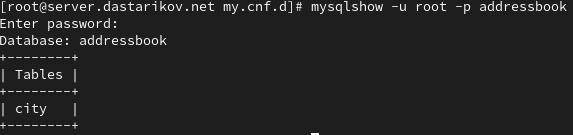
\includegraphics[width=\textwidth]{../images/image16.png}
    \captionof{figure}{Просмотр таблиц базы данных \texttt{addressbook} пользователем \texttt{root}.}
\end{frame}

\begin{frame}
\frametitle{Создание базы данных}
    \centering
    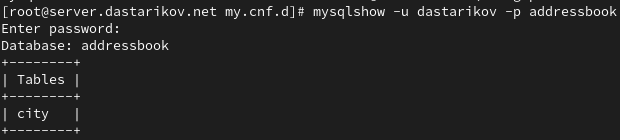
\includegraphics[width=\textwidth]{../images/image17.png}
    \captionof{figure}{Просмотр таблиц базы данных \texttt{addressbook} пользователем \texttt{dastarikov}.}
\end{frame}

\begin{frame}
\frametitle{Резервные копии}
    \centering
    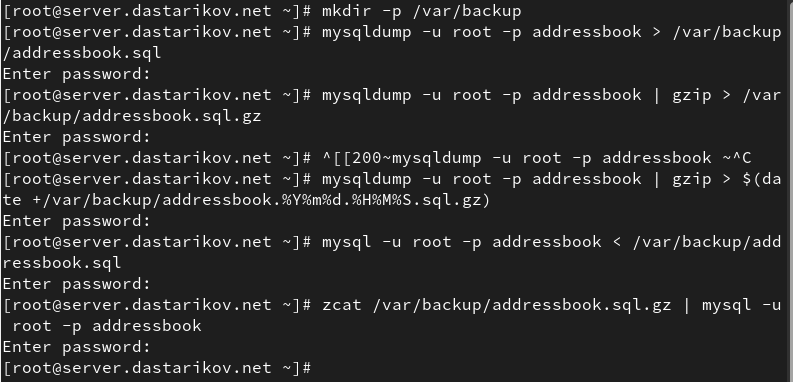
\includegraphics[width=\textwidth]{../images/image18.png}
    \captionof{figure}{Создание и восстановление резервной копии базы данных.}
\end{frame}

\begin{frame}
\frametitle{Внесение изменений в настройки внутреннего окружения виртуальной машины}
    \centering
    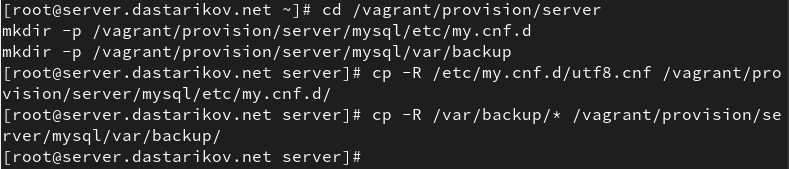
\includegraphics[width=\textwidth]{../images/image19.png}
    \captionof{figure}{Создание каталога для настроек внутреннего окружения.}
\end{frame}

\begin{frame}
\frametitle{Внесение изменений в настройки внутреннего окружения виртуальной машины}
    \centering
    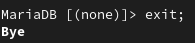
\includegraphics[width=\textwidth]{../images/image07.png}
    \captionof{figure}{Выход из интерактивной оболочки MariaDB.}
\end{frame}

\begin{frame}[containsverbatim]
\frametitle{Внесение изменений в настройки внутреннего окружения виртуальной машины}
  \begin{minted}[fontsize=\footnotesize]{bash}
    #!/bin/bash
    echo "Provisioning script $0"
    systemctl restart named
    echo "Install needed packages"
    dnf -y install mariadb mariadb-server
    echo "Copy configuration files"
    cp -R /vagrant/provision/server/mysql/etc/* /etc
    mkdir -p /var/backup
    cp -R /vagrant/provision/server/mysql/var/backup/* /var/backup
    echo "Start mysql service"
    systemctl enable mariadb
    systemctl start mariadb
  \end{minted}
\end{frame}

\begin{frame}[containsverbatim]
\frametitle{Внесение изменений в настройки внутреннего окружения виртуальной машины}
\begin{minted}[fontsize=\footnotesize]{bash}
    if [[ ! -d /var/lib/mysql/mysql ]]
    then
    echo "Securing mariadb"
    mysql_secure_installation <<EOF
    y
    123456
    123456
    y
    y
    y
    y
    EOF
    echo "Create database"
    mysql -u root -p123456 <<EOF
    CREATE DATABASE addressbook CHARACTER SET utf8 COLLATE utf8_general_ci;
    EOF
    mysql -u root -p123456 addressbook < /var/backup/addressbook.sql
    fi
\end{minted}
\end{frame}

\begin{frame}
\frametitle{Выводы}
\begin{itemize}
    \item В результате выполнения лабораторной работы приобрели практические навыки по установке и конфигурированию системы управления базами данных на примере программного обеспечения MariaDB.
\end{itemize}
\end{frame}
\end{document}
